\documentclass{article}
\usepackage[german]{babel}
\usepackage{cite}
\usepackage{url}
\usepackage{graphicx}

\author{Phillip Eckstein}
\title{Java Profiling}

\bibliographystyle{abbrv} 

\addto\captionsgerman{%
  \renewcommand{\contentsname}%
    {Inhalt}%
}


\begin{document}
    
\selectlanguage{german}
\maketitle
\tableofcontents

\pagebreak

\section{Einleitung}
Diese Arbeit beschäftigt sich mit dem Thema des Profilings in Java. Am Beispiel des Zuul Projektes wird der gesamte Vorgang des Profilings beschrieben. Dabei wird auf alle Wichtigen Aspekte der Auswahl und der Durchführung eingegangen. Als zu profilendes Projekt wird auf die Zuul Anwendung, welche im Modul Objektorientierte Softwareentwicklung der Westsächsisch Hochschule Zwickau erstellt wird zurückgegriffen. Dabei handelt es sich um ein Adventure Spiel. Die Besonderheit dieses Programms ist, dass es sowohl ueber eine Kommandozeile als auch mit einer Grafischen Benutzeroberfläche gespielt werden kann.Um eine Optimale Auswahl des Profilers zu gewährleisten, wird zuerst eine Anforderungsanalyse durchgeführt. Diese soll hervorheben welche Aspekte des Profilers für diese Arbeit von Bedeutung sind und welche ignoriert werden können. Die Profiler Auswahl soll einen Überblick geben, über die wichtigsten Java Profiler am Markt. Es wird auch darauf eingegangen warum welche Profiler unter Berücksichtigung der vorher in der Anforderungsanalyse aufgestellten Anforderungen geeignet sind und welche nicht. Danach wird das Profiling durchgeführt und dokumentiert. Dabei wird jeder Arbeitsschritt beschrieben und die Ergebnisse festgehalten. Anschließend wird eine Auswertung der Ergebnisse durchgeführt, um zu demonstrieren was man durch Profiling herausfinden kann.


\section{Begriffserklaerung}

Im Folgenden wird kurz auf eventuell unklare Begriffe eingegangen. Zunächst soll genauer definiert werden um was genau es sich bei Profilingh handelt. Als Profiling wird eine Tätigkeit beschrieben, bei der mit Hilfe von Programmen und Hilfsmitteln der Bytecode eines Programms, während er Ausführung überwacht wird. Dadurch lässt sich zum Beispiel der Speicherverbrauch und die Laufzeit der einzelnen Befehle besser ermitteln. Programme, die dafuer benutzt werden, werden Profiler genannt. Die beim Profilen gewonnenen Erkenntnisse sollen danach benutzt werden, um das Programm zu verbessern. Weiter für das Verständnis erforderlich sind folgende Begriffe:
IDE: Integraded Development Enviroment bezeichnet einen Texteditor mit integrierten Tools zum Komplizieren und Ausführen von Code.
Code: Nachfolgend wird der Programmtext der Anwendung auch als Code bezeichnet
GUI:  General User Interface  zu deutsch Grafische Benutzeroberflaeche
PID: Prozess Identifier zu deutsch Prozesskennung ~\cite{WEBSITE:6}

\section{Anforderungsanalyse}
Ein Profiler muss Anforderungen erfüllen. Diese ergeben sich abhängig von verschiedenen Einflüssen. Dazu zählen sowohl äußere Einflüsse als auch innere. Als äußere Einflüsse seien Einflüsse anzunehmen, die von ausserhalb der Softwareentwicklung stammen und nicht geändert werden können. Ein Beispiel dafür sind Unternehmensrichtlinien. Als interne Einflüsse sind Kriterien wie die Art, Programmiersprache und Architektur der zu profilenden Software sowie die benutzte IDE. Des Weiteren sollte schon im Voraus geklärt werden welche Teile der Anwendung genauer betrachtet werden sollen. Dies ist wichtig, da verschiedene Profiler wie nachfolgend beschrieben bestimmte Aspekte des Programms besser Testen können. An diese Stelle sei zu erwähnen, dass es wahrscheinlich nicht den einen Besten Profiler für das Projekt gibt, da die meisten Profiler in einem bestimmten Bereich besondere stärken haben. Es sit also durchaus herkoemmlich mehrere Profiler zu verwenden, abhaengig von den zu erwarteten Problemen. 


Im Rahmen dieser Arbeit soll eine Java Anwendung einem Profiling unterzogen werden. Als IDE kommt Intelij Ultimate von JetBrains zum Einsatz. Daraus ergibt sich bereits die erste  wenn auch sehr offensichtliche Anforderung: Es wird zwingend ein Profiler benötigt, der Java versteht. Eine weitere Anforderung ist, dass das Tool eine möglichst einfache Integration und Bedienung bietet, um unerfahreneren Anwendern das Arbeiten zu erleichtern. Da keine Server Applikation getestet werden soll werden Features wie Online-/ oder Fern-Profiling nicht benötigt. Auch enthält das Projekt keine Datenbank, welche man profilen könnte. Somit sind auch solche Funktionen für den Zweck dieser Arbeit nicht relevant. Eine Integration in die IDE kann jedoch von Vorteil sein, da so die Hürde genommen wird erst ein extra Programm zu starten und Profiling parallel zum Debugging durchgeführt werden kann. Dies führt dazu, dass mehr Bugs im Code gefunden werden können. Die zu Profilende Anwendung hat wie schon eingangs erwaehnt eine Besonderheit. das Spiel kann sowohl in der Kommandozeile als auch mit einem GUI ausgeführt werden.
Dies lässt einen anschaulichen Vergleich zwischen beiden Versionen zu. Eine Funktion, welche bei solch einem Vergleich von Vorteil sein könnte, ist das Erstellen von Abbildungen oder eine andere Form, die Ergebnisse speichern zu können und sie später vergleichen zu können.
Aber selbst der Beste Profiler nützt wenig, wenn man die Ergebnisse nicht sieht. Es ist also wichtig, dass Man schnell und auf einen Blick sieht, was vor sich geht. Der Profiler sollte also eine Gute Uebersichtsseite bieten. 

\section{Profiler-Auswahl}

Für das Profiling von Java stehen eine Vielzahl von Profilern zur Verfügung. ~\cite{Website:1} Diese werden nachfolgend genauer betrachtet und eine Auswahl auf Basis der in der Anforderungsanalyse betrachteten Kriterien getroffen.
Auf Grund der vielen verschiedenen Profiler kann leider kein Anspruch auf Vollständigkeit gestellt werden, da auch immer wieder neue auf den Markt kommen. Zur Auswahl stehen sowohl kostenfreie als auch kostenpflichtige Optionen. Einige der Profiler sind Bestandteil anderer Anwendungen wie IDEs, wenn dies der Fall wird ausschließlich der für den Profiler relevante Teil betrachtet. Nachfolgend eine kurze Vorstellung der Profiler sowie ein Tabellarischer Vergleich. \ref{tab:1}

\paragraph{JProfiler}

soll Als erstes betrachtet werden. Bei diesem Tool handelt es sich um eine eigenständige Applikation, welche von ej-Technologies entwickelt wird ~\cite{WEBSITE:2} Sie gilt als eine der am häufigsten benutzen Profiler für Java. ~\cite{WEBSITE:3} JProfiler bietet die Möglichkeit Snapshots, also Momentaufnahmen aller aktuellen Profiling Daten zu erstellen und zu speichern. Außerdem bietet es verschiedene Möglichkeiten Aufnahmen des gleichen Programms zu vergleichen. Weitere Funktionen sind unter anderem die Auswertung von Datenbanken und APIs wie JPA. JProfiler ist eine Kostenpflichtige Anwendung, bei der die moeglichkeit besteht, sich fuer eine kostenlose Open-Source Lizenz zu registrieren.

\paragraph{YourKit}
ist ebenfalls eine eigenständige Anwendung. Sie wird von der gleichnamigen YourKit GmbH entwickelt ~\cite{WEBSITE:4} YourKit Bietet die Möglichkeit sowohl .NET als auch Java Anwendungen zu Profilen. Es unterstützt sowohl lokales als auch remote Profiling und bietet eine gute Integration in Intellij sowie andere IDEs. Des Weiteren gibt es die Möglichkeit Snapshots, also Momentaufnahmen des Arbeitsspeichers und der CPU-Prozesse zu erstellen und mit anderen zu vergleichen. Ein herrausstellungsmerkmal ist der Sogenante Flame-Graph welcher Prozesszeiten sehr anschaulich darstellt. Weitere Funktionen sind das Profilen von Datenbankabfragen sowie das Profilen von Exceptions. YourKit ist ebenfalls kostenpflichtig, bietet aber Testversionen und Open-Source Lizenzen.

\paragraph{Java VisualVM}

ist ein Tool, welches einige Zeit zusammen mit Oracle Java ausgeliefert wurde. ~\cite{WEBSITE:5} Aktuell wird es als eigenständige Anwendung vertrieben. Es unterstützt alle grundlegenden Methoden des Profilings. Eine Besonderheit ist, dass man es über Plugins erweitern kann. Das ermöglicht es, für die eigene Software maßgeschneiderte Profiler zu integrieren. Java VisualVM ist kostenlos.

\paragraph{Tabellarischer Vergleich}

Nachfolgend der Tabellarische Vergleich zwischen den drei Profilern. 
\begin{table}[h]
  \centering
  \caption{Vergleich von Java Profilern}
  \begin{tabular}{cccc}
    Kriterium & JProfiler & YourKit & Java VisualVM\\
    \hline
    Java Kompatibel & Ja& Ja & Ja\\
    Lokales Profiling &Ja&Ja&Ja\\
    Remote Profiling&Ja&Ja&Ja\\
    Intellij Integration&Ja&Ja&Ja\\
    Speicherprofiling&ja&ja&ja\\
    Prozessprofiling&ja&ja&ja\\
    Snapshot Vergleich&ja&ja&nein\\
    Gute visuelle Darstellung &ja&nein&nein\\
    Erweiterbarkeit&nein&nein&Ja
  \end{tabular}
  \label{tab:1}
\end{table}

\paragraph{Auswahl}
Nach Auswertung der Erkenntnisse über die einzelnen Profiler wurde sich für Java VisualVM entschieden.  Grund dafür waren neben den Kosten vor allem das einfach zu verstehende UI sowie die Einfachheit der Anwendung. Da die einfach zu verstehende UI aber ein doch recht subjektives Kriterium ist sei an dieser Stelle einmal angemerkt, dass für den Zweck dieser Arbeit die meisten Profiler alle Anforderungen mehr als ausreichend erfüllen. Die Unterschiede liegen hier wie so oft im Detail. VisualVM bietet zwar die insgesammt wenigsten moeglichkeiten, ist aber fuer den zweck dieser Arbeit foellig ausreichend, da die meisten der Zusatzfunktionen der anderen Profiler nicht benoetigt werden. 

\section{Durchfuehrung}
Als erstes muss VisualVM heruntergeladen und installiert werden. Den Download-Link kann man unter Downloads auf Der Hauptseite von VisualVM finden. Nachdem der Zip komprimierte Ordner heruntergeladen wurde muss dieser noch entpackt werden und an eine passende Stelle im Nutzerverzeichnis verschoben werden. Da zur Entwicklung der Software Intellij benutzt wird soll der Profiler als nächstes in dieses Integriert werden. Dazu ist es nötig das Plugin VisualVM Launcher von VojTech Krasa zu installieren. Dieses Plugin fügt Buttons zum Starten des Profiling-Vorgangs mit VisualVM hinzu. ~\cite{fig:Intellij_VisualVM_Button}
\begin{figure}[t]
  \centering
  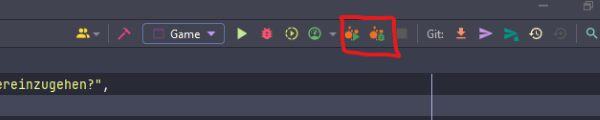
\includegraphics{Intellij_VisualVM_Button}
  \caption{Die neuen Profiling Buttons in Intellij}
  \label{fig:Intellij_VisualVM_Button}
\end{figure}
Bei ersten Starten ist es notwendig den Pfad zu der gerade entpackten, ausführbaren Datei von VisualVM anzugeben. diese befindet sich normalerweise im gerade entpackten Verzeichnis unter /bin. Um das Profilen der Anwendung zu starten, reicht es also aus anstelle des Ausführen-Buttons den Profiler Buttons zu drücken. Nachdem Der Profiler gestartet ist wird man von der Startseite begrüßt. ~\cite{fig:VisualVM_MainPage} Von hier aus kann man sich anzeigen lassen wieviel last das Programm auf der CPU verursacht, wieviel Speicher verbraucht wird und welche Methoden ausgeführt werden. Der Overview Tap liefert allgemeine Informationen wie die PID, wo das Programm ausgeführt wird, wie die Hauptklasse heißt und welche Java 
VM benutz wird. Der Monitor Tab liefert aktuelle daten in grafisch aufbereiteter form über CPU last, Heap Größe, geladene Klassen und aktive Threads.
Der Threads Tab gibt eine Timeline mit allen zu einem bestimmten Zeitpunkt ausgeführten Threads. Diese sind farblich kodiert, um die verschiedenen Zustände anzuzeigen. Außerdem sind Die Laufzeit und die Gesamtheit, die jeder Thread aktiv war zu sehen. Der Letzte Tab enthält die Sampling Funktionen. Diese ermöglichen es Aufnahmen von CPU und Speicher zu erstellen um diese später auswerden zu können. Diese Aufnahmen sind das eigentliche Profilen. VisualVM bietet hier zwei Möglichkeiten. die Erste ist das Samplen der CPU. Dabei wird der Callstack des Programms sowie sie Ausführzeit der einzelnen Threads aufgezeichnet. Man kann dabei sowohl Momentaufnahmen tätigen als auch das ganze nach beenden als Datei speichern. Ähnlich funktioniert das Memory Profilen. Hier wird stattdessen aber aufgezeichnet welche Objekte wieviel Speicher verbrauchen. Nachdem nun alle Grundfunktionen erklärt sind kommen wir zum interessanten teil, des profiliens der eigentlichen Anwendung.

\paragraph{Komandozeilenanwendung}
Als erstes soll die Konsolenversion des Spiels geprofiled werden. Dies geschieht, indem die main-Methode der Klasse Game ausgeführt wird. Nachdem das Programm gestartet ist, wird der Monitor Tab geöffnet. Das Programm wird vorerst ohne Eingabe, sozusagen im Idle laufen gelassen und es wird beobachtet, wie sich die Graphen verhalten. Es ist zu beobachten das sich die Applikation langsam aber stetig mehr Speicher einverleibt. So beträgt der Speicherbedarf der Applikation zum Start 6,385 MB. Nach 2 Minuten im Idle zustand betrug der Speicherbedarf im test 21,065MB. Der Speicherbedarf stieg so lange an bis manuell über VisualVM die Garbage Collection betätigt wurde. Dies reduzierte sowohl die maximale Heap Größe als auch die genutzte Größe. danach änderte sich auch das Verhalten im idle. So stieg der Speicher bedarf nicht erneut auf über 30MB, sondern wurde nach ca. 5 Minuten wieder weniger. CPU last, Klassen und Threads waren hingegen uninteressant. Hier ließ sich kein interessantes Verhalten beobachten.
Anschließend wurde das Spiel über die Kommando Zeile einmal durchgespielt, einmal mit CPU-Sampling und einmal mit Speichersampling. Beide Ergebnisse wurden gespeichert, um sie mit der Grafischen Oberfläche zu vergleichen.

\paragraph{GUI Anwendung}
Als zweites wurde die Grafische Benutzeroberfläche geprofiled. Vorgegangen wurde dabei genauso wie bei der Kommandozeile, um die Ergebnisse Vergleichbar zu halten. Auch hier konnte man direkt einen Speicherbedarfszuwachs erkennen. Allerdings fiel der Speicherbedarf nach ca. 7 Minuten von allein schlagartig, um danach wieder anzusteigen. Nach einiger Zeit begann der Speicherverbrauch Schlagartig rapide zu steigen und viel in kürzeren Zeitfrequenzen wieder schlagartig. Die Applikation startete mit einem Speicherverbrauch von 25,478MB und stieg über eine Zeit von ca. 6 Minuten auf 82,108MB an. Danach fiel sie schlagartig auf 22,365MB. Im weiteren Verlauf von 2 Minuten stieg der Speicherbedarf wieder leicht, nur um dann rapide innerhalb 30 Sekunden von ca. 39MB auf 116,373MB anzusteigen. Über die nächsten 8 Minuten wiederholten sich diese Spitzen mit zunehmender Amplitude uns Sinkender Frequenz immer weiter. Auch die CPU last zeigte Unterschiede. Ungefähr zum selben Zeitpunkt, an den die Speicherspitzen auftraten, kann man erkennen das die CPU-Aktivität zugenommen hat. Diese war zwar immer noch sehr gering, aber erkennbar. Der Spitzenwert beträgt in diesem Test 3,2\% CPU-Last. Anschließend wurde das Spiel über das GUI einmal durchgespielt, einmal mit CPU-Sampling und einmal mit Speichersampling. Beide Ergebnisse wurden ebenfalls gespeichert.



\section{Auswertung und Fazit}
\paragraph{Auswertung}
Als erstes wird der Idle Test ausgewertet. Das Verhalten beider Versionen der Zuul Applikation ist sehr unterschiedlich. Neben dem erwartet höheren Speicherverbrauch der GUI legt diese ein gänzlich anderes Verhalten an den Tag. Aufgrund Der GUI ist ein höherer Speicherverbrauch zu erwarten, da mehr Daten geladen werden müssen. Die Aufgenommenen Samples Des Ausführungstests geben Aufschluss über die Ausführungszeit der einzelnen Methoden. Dabei ist aber kaum ein Unterschied zwischen GUI und Kommandozeile zu erkennen, was daran liegt das meist die Exakt selben Methoden ausgeführt werden. lediglich die Methoden für die Eingabe sind andere. Hier fällt die InitializeFight Methode auf, welche in Kommandozeilenanwendung mit 15ms eine erheblich längere Ausführdauer hat. Dies ist aber damit zu erklären das in dieser Methode der Parser Modus gewechselt wird, um die Kampf Kommandos parsen zu können, was im GUI umgangen werden kann.

\paragraph{Fazit}
Profiling ist ein gutes Hilfsmittel, um Perfomance Problemen auf die Spur zu kommen. In Java ist es dank einer Vielzahl an Tools für viele verschiedene Anwendungszwecke leicht zu realisieren. Es gibt Aufschluss über die Laufzeit und den Speicherbedarf der Anwendung. So kann man analysieren welche Methoden besonders lang benötigen oder ob es eventuell Speicherlecks gibt. Die Kenntnisse, die bei der Durchführung eines Profilings gewonnen werden, können direkt für das Verbessern der Anwendung benutzt werden. Profiling fordert aber ein gewisses Grundwissen über die Funktionsweise von Speicher, Speicherverwaltung sowie des Schedulings, um die Probleme Korrekt erkennen zu können.

\bibliography{Quellen}

\pagebreak
\section{Abbildungen}
\begin{figure}[h]
  \centering
  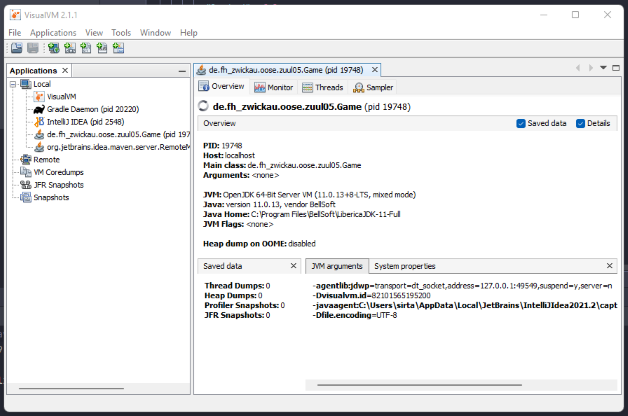
\includegraphics{VisualVM_StartPage.png}
  \caption{Hauptansicht von VisualVM}
  \label{fig:VisualVM_MainPage}
\end{figure}

\begin{figure}
  \centering
  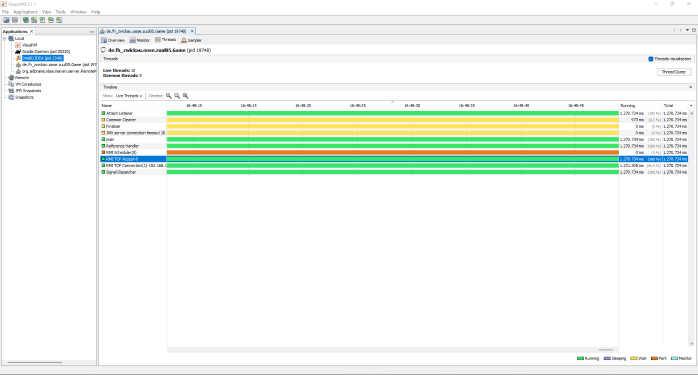
\includegraphics{VisualVM_Threads.png}
  \caption{Thread Ansicht von VisualVM}
  \label{fig:VisualVM_Threads}
\end{figure}

\begin{figure}
  \centering
  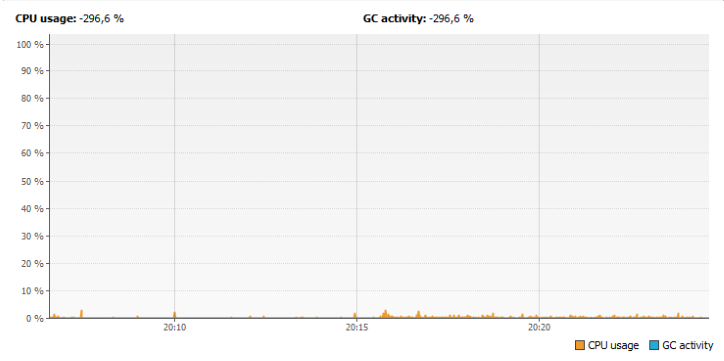
\includegraphics{GUI_CPU_idle.png}
  \caption{CPU auslastung der GUI im Idle zustand}
  \label{fig:GUI_CPU_idle}
\end{figure}

\begin{figure}
  \centering
  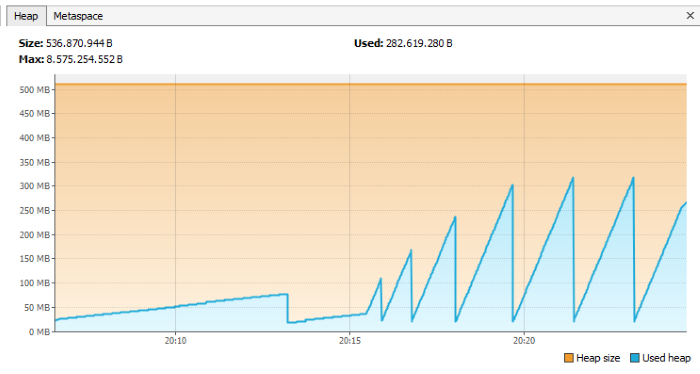
\includegraphics{GUI_Idle.png}
  \caption{Speicherbedarf auslastung der GUI im Idle zustand}
  \label{fig:GUI_MEM_idle}
\end{figure}

\begin{figure}
  \centering
  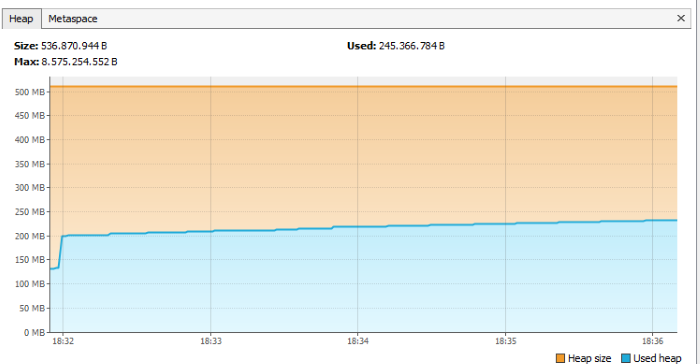
\includegraphics{Memory_console_execute.png}
  \caption{Speicherbedarf der Konsole waerend des Spieldurchgangs}
  \label{fig:Console_mem_Execute}
\end{figure}
\end{document}
